\documentclass[a4paper,12pt]{ltjsarticle}
\usepackage{luatexja}
\usepackage{graphicx}
\usepackage{amsmath, amssymb}
\usepackage{geometry}
\geometry{margin=25mm}

\begin{document}

\begin{titlepage}
  \centering
  {\large 千葉工業大学 東本研究室 \part}
  {\large 進捗報告書 \par}
  \vspace{1.5cm}
  {\Huge \bfseries 進捗報告 Ver.25 \par}
  \vspace{1cm}
  \rule{0.7\textwidth}{0.5pt} \par
  \vspace{1cm}
  {\Large 内山 裕太 \hspace*{1cm} \today \par}
  \vspace{3cm}
  \thispagestyle{empty}
\end{titlepage}

\section{今週実施したこと}
\begin{itemize}
  \item ALST原稿執筆
  \item 紫関君実験リハ
  \item 高野君実験リハ
  \item LaTeX環境の構築(バカむずい)
  \item ポスターの土台制作
  \item 考えの整理
\end{itemize}
\clearpage

\section{実施事項の詳細}
\textbf{ALST原稿執筆}\par
東本先生,古池先生のご協力もあり,執筆完了.\\

\textbf{紫関君実験リハ}\par
前回のメンターリハ以降の動きが確認できていない\par
10/17(金)にSlack上で状況確認中\\

\textbf{高野君実験リハ}\par
10/16(木)に先生リハを実施(MTGになった感じ)\par
高野君が考える概念と先行研究の概念の相違や,実験内における表現など修正点がいくつか現れた.修正後にメンターで確認を行い,先生MTGを通しながら実験リハを目指す方向性で考えている.
システムの修正などは大きく時間がかかるわけではなさそう.\\

\textbf{LaTeX環境の構築}\par
白髭先輩から修論のプレみたいなやつをもらった\par
めっちゃ面倒だったけど慣れた\\

\textbf{ポスターの土台制作}\par
過去の先輩を参考に土台だけ作ってみました(添付資料)
\clearpage

\section{来週やること}
begin{itemize}
  \item 体調を治す
  \item ポスターの完成
  \item 目標設定(技術,人間)
\end{itemize}

\section{現状の問題点}
\begin{itemize}
  \item 寒い
  \item 自分に合ったスケジュールと目標を立てられてない
\end{itemize}

\section{スケジュール}
\begin{center}
  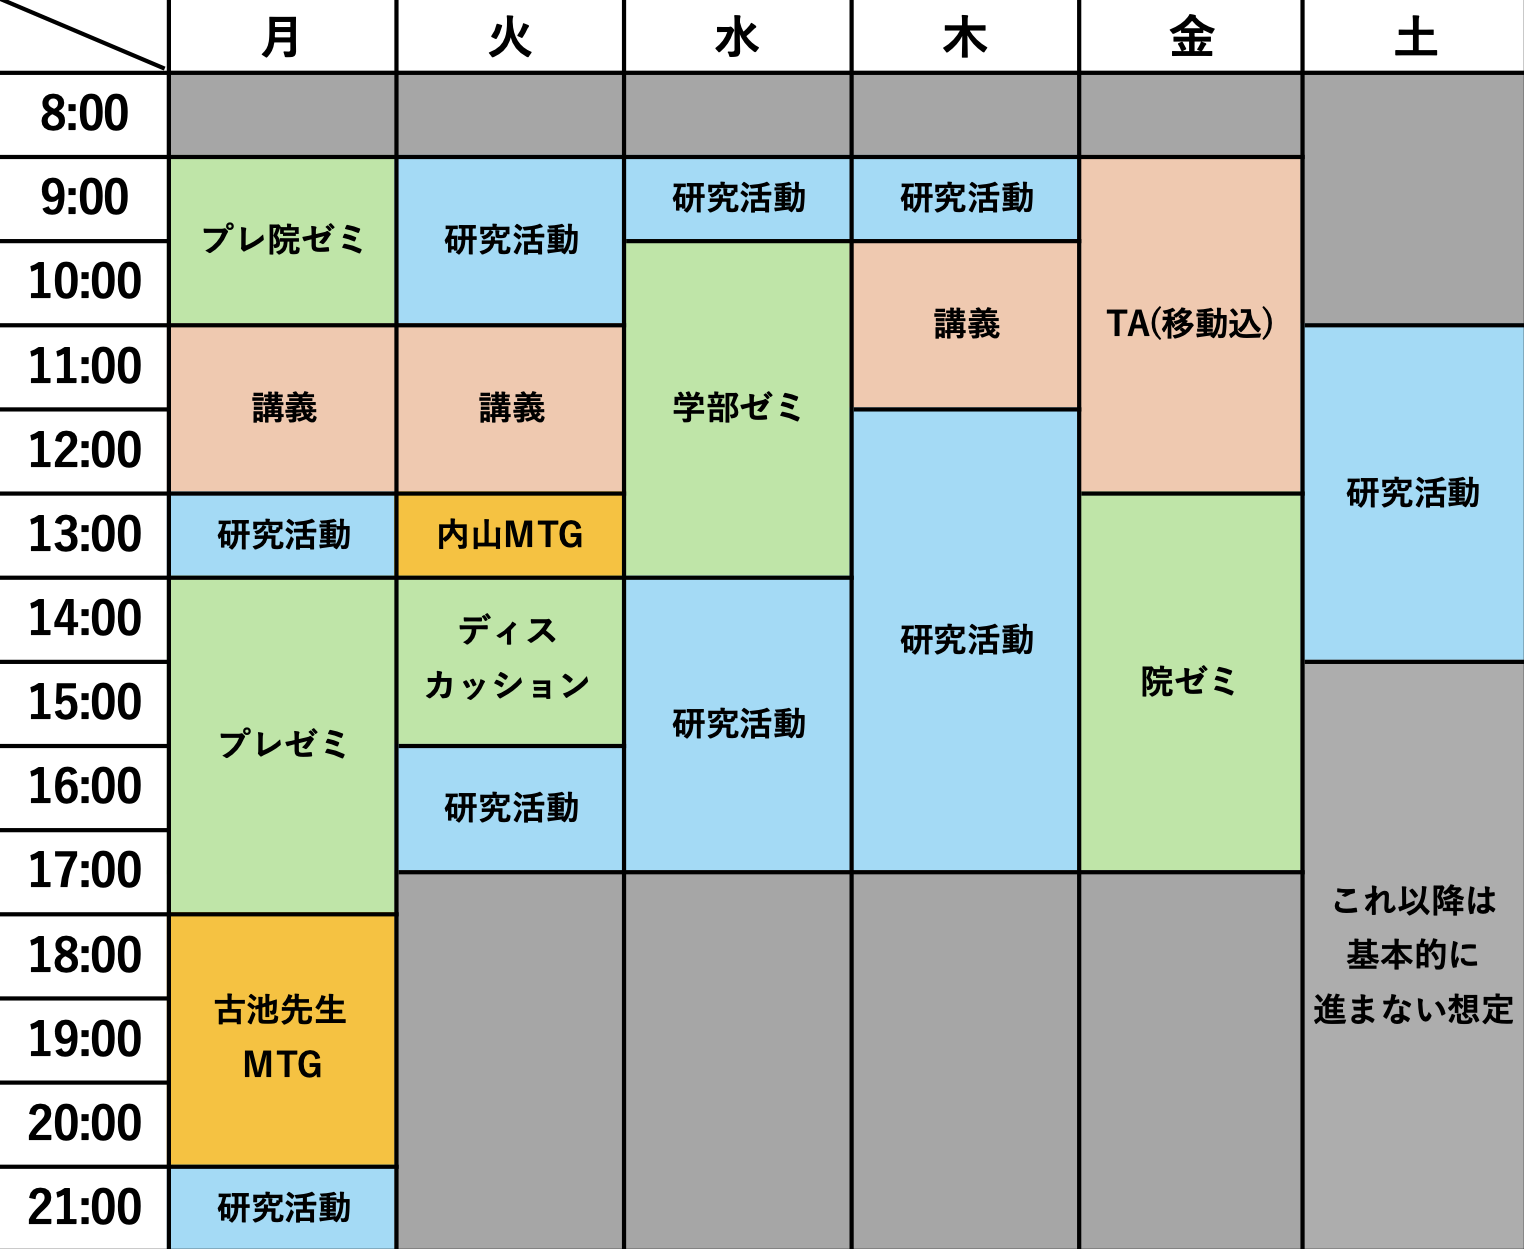
\includegraphics[width=0.8\textwidth]{figs/2025_2_schedule.png}
\end{center}

\section{メンター関係}
\begin{itemize}
  \item Notionに記載
\end{itemize}
\clearpage

\section{雑談}
$y = x$みたいな感じで、行中に埋め込めますし、以下のように書くこともできます。\\

\begin{equation}
  \int_{a}^{a}f\left(x\right)dx = 0
\end{equation}

複数行の数式も書けます。$=$の位置を揃えることもできます。\\

\begin{align}
  \int_{1}^{2}\left(x^2 + 3x\right)dx + \int_{1}^{2}\left(x^2 - 3x\right)dx &= \int_{1}^{2}\left\{\left(x^2 + 3x\right) + \left(x^2 - 3x\right)\right\}dx \\
  &= \int_{1}^{2}2x^2dx \\
  &= 2\left[\frac{x^3}{3}\right]^2_1 = \frac{2\left(2^3 - 1^3\right)}{3} = \frac{14}{3}
\end{align}

\end{document}